\section{Mediator}


Nesse padrão, um objeto chamado de \textit{Mediator} age como intermediário 
entre um grupo de objetos, ficando responsável por qualquer 
interação entre eles. O \textit{Mediator} conhece todos 
esses objetos enquanto cada objeto conhece apenas o 
\textit{Mediator}, o que os torna 
mais independentes, simplificando sua reutilização
 e concentrando as dependências entre eles 
em um só lugar. \cite{gamma:1995}

A estrutura do padrão é apresentada na Figura \ref{mediator_struct}. 
Uma interface \texttt{Mediator} define as operações que um tipo de 
objeto \textit{Mediator} deve possuir. \texttt{ConcreteMediator} representa 
uma classe que implementa essas operações. Um \texttt{Colleague} 
é um objeto conhecido pelo \texttt{Mediator} e cada \texttt{ConcreteColleague} 
pode ser tanto um objeto que possui operações refletidas 
em outros objetos quanto ser um dos objetos afetados 
indiretamente por outro \texttt{Colleague}.

\begin{figure}[htb]
	\caption{\label{mediator_struct}Estrutura do \textit{Mediator}.}
	\begin{center}
	    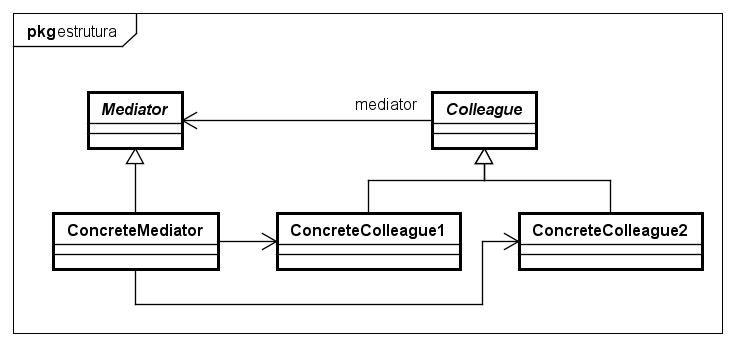
\includegraphics[scale=0.5]{5_padroes-contexto-funcional/5.3_comportamentais/5.3.05_mediator/mediator_estrutura.png}
	\end{center}
  \caption*{Fonte: O Autor (2021)}
\end{figure}

\subsection*{Exemplo Orientado a Objetos}

Como exemplo, é considerada uma janela de uma aplicação 
que apresenta diversos \textit{widgets}, entre eles uma caixa 
de entrada de texto e uma lista de seleção. Quando um item é 
selecionado na lista, o texto contido nele deve aparecer 
na caixa de entrada de texto. O \textit{Mediator} é responsável 
por alterar a caixa de entrada de texto quando um item 
é selecionado na lista, enquanto a lista é responsável 
por informar ao \textit{Mediator} quando um item for selecionado. 
A Figura \ref{mediator_exemplo} apresenta o diagrama 
de classes para esse exemplo. O Código \ref{oomediator} 
apresenta a implementação do padrão para esse exemplo.

\begin{figure}[htb]
	\caption{\label{mediator_exemplo}Exemplo de \textit{Mediator}.}
	\begin{center}
	    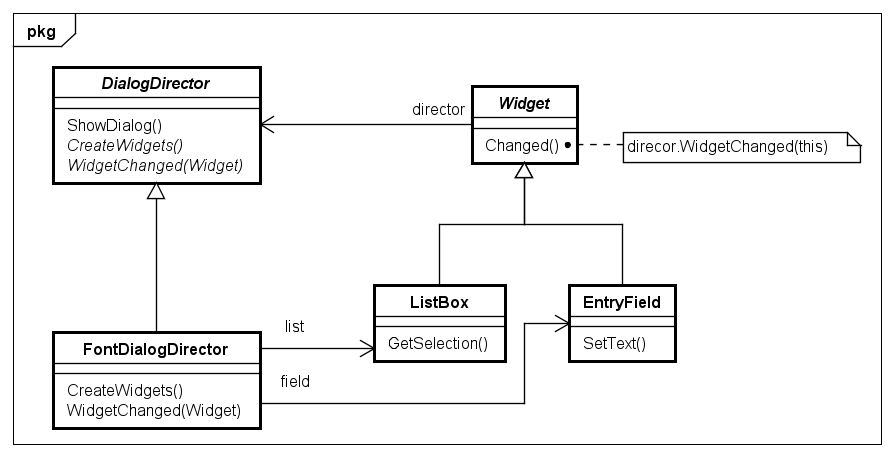
\includegraphics[scale=0.5]{5_padroes-contexto-funcional/5.3_comportamentais/5.3.05_mediator/mediator_exemplo.png}
	\end{center}
  \caption*{Fonte: O Autor (2021)}
\end{figure}

\begin{lstlisting}[caption={\textit{Mediator} Orientado a Objetos.},label=oomediator]

abstract class DialogDirector {

  def ShowDialog() : Unit = {
    //Exibe o dialog
  }

  def CreateWidget()
  def WidgetChanged(widget: Widget)
}

class FontDialogDirector() extends DialogDirector {

  private var list : ListBox = null
  private var field : EntryField = null

  override def CreateWidget(): Unit = {
    this.list = new ListBox(this)
    this.field = new EntryField(this)
  }

  override def WidgetChanged(widget: Widget): Unit = {
    this.field.text = this.list.selection
  }
}

abstract class Widget(val director : DialogDirector) {
  def Changed() : Unit = director.WidgetChanged(this)
}

class EntryField(director : DialogDirector) extends Widget(director) {
  var text : String = ""
}

class ListBox(director : DialogDirector) extends Widget(director){
  private var _selection : String = ""
  def selection : String = _selection

  def SetSelection(selection : String) : Unit = {
    this._selection = selection
    Changed()
  }
}
    
\end{lstlisting}
\legend{Fonte: O Autor (2021)}

\subsection*{Contexto Funcional}

O Código \ref{fpmediator} demonstra a implementação 
funcional do \textit{Mediator}. Uma função é responsável por 
gerenciar as interdependências entre os valores 
dos tipos \texttt{EntryField}, definido na linha 2, e \texttt{ListBox}, 
definido na linha 12. Quando a função mediadora \texttt{ChangeSelection}, 
definida na linha 22, é chamada, ela precisa receber 
como parâmetro o elemento alvo e o elemento dependente, 
além das informações necessárias para executar a 
operação \texttt{ChangeListBoxSelection}. A função retorna 
tanto o \textit{colleague} alvo da operação 
quanto os \textit{colleagues} afetados, mantendo 
a função cliente que chama essa operação atualizada 
quanto ao estado de ambos os valores. 

A vantagem dessa abordagem é que ela torna possível 
que as funções dos \textit{colleagues} (no Código 
\ref{fpmediator}, \texttt{ChangeEntryFieldText} e 
\texttt{ChangeListBoxSelection}) sejam idependentes dos 
mediadodores, favorecendo seu reuso. A desvantagem 
é que é necessário realizar, na função cliente, 
um gerenciamento quanto ao estado de todos os 
\textit{colleagues}, já que a função mediadora 
deve ser pura e não realiza efeitos colaterais.

\begin{lstlisting}[caption={\textit{Mediator} Funcional.},label=fpmediator]
    
type EntryField = String

def ChangeEntryFieldText(text : String,
						 entryField: EntryField)
: EntryField =
  text
  
def GetText(entryField : EntryField) : String =
  entryField
  
type ListBox = String
  
def ChangeListBoxSelection(selection : String,
						   listBox: ListBox)
: ListBox =
  selection
  
def GetSelection(listBox : ListBox)  : String=
  listBox
  
def ChangeSelection(selection : String,
					entryField: EntryField,
					listBox : ListBox) : (EntryField, ListBox) = {
  (ChangeListBoxSelection(selection, listBox), ChangeEntryFieldText(selection, entryField))
}
	    
\end{lstlisting}
\legend{Fonte: O Autor (2021)}